\documentclass{beamer}
\usepackage{gtu-presentation}
\usepackage[style=ieee]{biblatex}
\addbibresource{bitirme.bib}
\usepackage{csquotes}% Needed for babel(in biblatex)
\usepackage[english]{babel}
\usepackage{amssymb}
\usepackage{xcolor}
\usepackage{amsmath}
\usepackage{graphicx}
\usepackage{tikz}
\usepackage{float}
\usepackage{subfig}
\setbeamertemplate{itemize item}[circle]
\usepackage{tabularx}
\definecolor{lightgreen}{HTML}{008000}

\newcommand\ytl[2]{
\parbox[b]{9em}{\hfill{\color{cyan}\bfseries\sffamily #1}~$\cdots\cdots$~}\makebox[0pt][c]{$\bullet$}\vrule\quad \parbox[c]{8cm}{\vspace{8pt}\color{red!40!black!80}\raggedright\sffamily #2.\\[7pt]}\\[-3pt]}
\newcommand*\circled[1]{\tikz[baseline=(char.base)]{
\node[shape=circle,draw,inner sep=1pt] (char) {#1};}}
\begin{document}
 
\begin{frontpage}
  \title{Minimum k-Chinese Postman Problem}
  \author{Akif Kartal}
  \date{15 June 2022}
  \advisor{Prof. Dr. Didem GÖZÜPEK}
\end{frontpage}



\begin{projectdefinition}
  	\begin{columns}[c] % The "c" option specifies centered vertical alignment while the "t" option is used for top vertical alignment
		
		\column{.50\textwidth} % Left column and width
		\begin{figure}
		    \centering
		    \includegraphics[width=2.1in,height=1.3in]{images/posttt.png}
		    \includegraphics[width=2.1in,height=1.3in]{images/ert.jpg}
		    \label{fig:widerface5}
	    \end{figure}
	  
\column{.50\textwidth}
Given a multigraph $G = (V,E)$ initial vertex $s \in V$ length $l(e) \in N$ for each $e \in E$ the \textit{minimum k-Chinese postman problem} is to find \textit{k} tours(cycles) such that each containing the initial vertex \textit{s} and each edge of the graph has been traversed at least once and the most expensive tour is minimized.\cite{book1}
\end{columns}
\end{projectdefinition}

\begin{result}
 
        
		\begin{figure}
		\begin{itemize}
        \item Making literature research and understanding the problem.
		\item Choosing and designing algorithms.
		\item Implementing both heuristic and exhausted search algorithms.
		\item Making complexity analysis of the algorithms.
		\item Testing with different parameters and performance evaluation.
		\item Making comparison and numerical evaluation of algorithms.
		\item Showing the comparison average results on the charts.
		\item Creating a GUI and running algorithms on that GUI.
\end{itemize}
            \vspace{0.03\textheight}
		    \includegraphics[width=2in,height=1in]{images/did.png}
		    \label{fig:widerface}
	    \end{figure}
		
\end{result}

\begin{projectrequirements}
In order to make this project, I have used following tools and technologies.
\vspace{0.02\textheight}
	\begin{figure}
		    \centering
		    \includegraphics[width=4in,height=2in]{charts/techss.png}
		    \label{fig:widerface5}
	\end{figure}

\end{projectrequirements}

\begin{projectdesign}
	In order to solve this problem, I have implemented a heuristic augment-merge algorithm.\cite{book7} Steps of this algorithm are following.
    \vspace{0.02\textheight}
	\begin{enumerate}
	 \item Sort the edges e in decreasing order according to their weight.
        \vspace{0.02\textheight}
		\item In decreasing order according to $ w(C_{e}) $, for each $e = {v_{i}, v_{j}} \in E $, create the closed walk $C_{e} =$ $(SP(v_{1}, v_{i})$, $e, SP(v_{j}, v_{1}))$, if \textit{e} is not already covered by an existing tour.
		\vspace{0.02\textheight}
		\item  Let $C = (C_{1}$, ... ,$C_{m})$ be the resulting set of tours. If $m = k$ we are done and have computed an optimal \textit{k }-postman tour. 
		\vspace{0.02\textheight}
		\item If $m < k$ we add $\textit{k} - \textit{m}$ “dummy” tours to \textit{C}, each consisting of twice the cheapest edge incident to the depot node.
\vspace{0.02\textheight}
		\item While $|C| > k$ we merge tour $ C_{k+1} $ with a tour from $C_{1}, ... ,C_{k}$ such that the weight of the merged tour is minimized.
	\end{enumerate} 
	 

	
  
		
\end{projectdesign}


\begin{projectrequirements3}
    \begin{table}[!htbp]
    \begin{flushleft}
    \textbf{*} $n = |E|$
    \vspace*{0.15cm}
    \end{flushleft}
    \centering
    \begin{tabular}{| m{2cm} | m{8cm} |} 
        \hline
        \textbf{\centerline{Complexity}} & \textbf{\centerline{Algorithm Step}} \\
        \hline
        \hspace*{\fill} $\mathcal{O}(n^2)$ \hspace*{\fill} & Sort the edges e in decreasing order according to their weight.\\ 
        \hline
        \hspace*{\fill} $\mathcal{O}(n^3)$ \hspace*{\fill} & For each $e = {v_{i}, v_{j}} \in E $, create the closed walk.\\ 
        \hline
        \hspace*{\fill} $\mathcal{O}(n^2)$ \hspace*{\fill} & If number of cycle(m) $< k$ add $\textit{k} - \textit{m}$ “dummy” tours.\\ 
        \hline
        \hspace*{\fill} $\mathcal{O}(n^4)$ \hspace*{\fill} & If number of cycle(m) $> k$ merge tour $ C_{k+1} $ with a tour from $C_{1}, ... ,C_{k}$.\\ 
        \hline
    \end{tabular}
    \caption{\label{tab:heru}Complexity Analysis of Heuristic Algorithm Steps}
    \textbf{Overall Complexity of Heuristic Algorithm} \\
    \vspace{0.015\textheight}
\textit{Best Case:} $\mathcal{O}(n^3)$ \\
\textit{Average Case:} $\mathcal{O}(n^3)$ \\
\textit{Worst Case:} $\mathcal{O}(n^4)$ 
\end{table}

			    
\end{projectrequirements3}



\begin{chart3}

   In this project, \textbf{to make a comparison}, we need to implement another algorithm. For this purpose, I have implemented a simple exhaustive search algorithm. Steps of this algorithm are as follows.
\vspace{0.02\textheight}
\begin{enumerate}
        \item Firstly, it finds all possible cycles in a graph by using a simple recursive algorithm like Depth-first search.\cite{ten}
        \vspace{0.015\textheight}
        \item Then, for the cycles found in the previous step, it finds all distinct combinations of a given length k.\cite{eleven} \\
        \centerline{C(all possible cycles, k)} 
        \vspace{0.015\textheight}
        \item Then, it finds all set of cycles that satisfy and holds the problem conditions in found combinations.
        \vspace{0.015\textheight}
        \item Lastly, we choose the k cycle that has a minimum length in set of cycles that have been found in the previous step.
\end{enumerate}
			    
\end{chart3}

\begin{chart5}
    \begin{table}[!htbp]
    \begin{flushleft}
    \textbf{*} $m = |V|, n = |E|$
    \vspace*{0.15cm}
    \end{flushleft}
    \centering
    \begin{tabular}{| m{3cm} | m{7cm} |} 
        \hline
        \textbf{\centerline{Complexity}} & \textbf{\centerline{Algorithm Step}} \\
        \hline
        \hspace*{\fill} $\mathcal{O}(m + n)$ \hspace*{\fill} & Finding all cycles in undirected graphs.\cite{book8} \\ 
        \hline
        \hspace*{\fill} $\mathcal{O}(n!)$ \hspace*{\fill} & Find all k combinations of found cycles in the previous step. \cite{eleven}\\ 
        \hline
        \hspace*{\fill} $\mathcal{O}(n^3)$ \hspace*{\fill} & Finding all cycles that satisfy the problem conditions in found combinations.\\
        \hline
        \hspace*{\fill} $\mathcal{O}(n^4)$ \hspace*{\fill} & Choosing the cycle that has a minimum length in cycles that have been found.\\ 
        \hline
    \end{tabular}
    \caption{\label{tab:widgets3}Complexity Analysis of Exhaustive
Search Algorithm Steps}
    \textbf{Overall Complexity of Exhaustive Search Algorithm} \\
    \vspace{0.02\textheight}
\textit{Best Case:} $\mathcal{O}(n!)$ \\
\textit{Average Case:} $\mathcal{O}(n!)$ \\
\textit{Worst Case:} $\mathcal{O}(n!)$ 
\end{table}

			    
\end{chart5}


\begin{projecttimeline2}

In this comparison, we will change the both number of nodes and the number of edges which means we will have a bigger graph. The k value will be constant. We will create \textbf{20 different graphs} and we will compare the average of the results.
\newline
\newline
Parameters will be as follows.
\vspace{0.03\textheight}
\begin{itemize}
 \item \textbf{initial vertex} = 0 
 \vspace{0.02\textheight}
 \item \textbf{k} = 3
 \vspace{0.02\textheight}
 \item \textbf{number of nodes} = 4, 5, 6, 7, 8
 \vspace{0.02\textheight}
 \item \textbf{number of edges} = 6,9,10,12,12
\end{itemize}
 
\end{projecttimeline2}

\begin{projecttimeline3}

\begin{figure}
    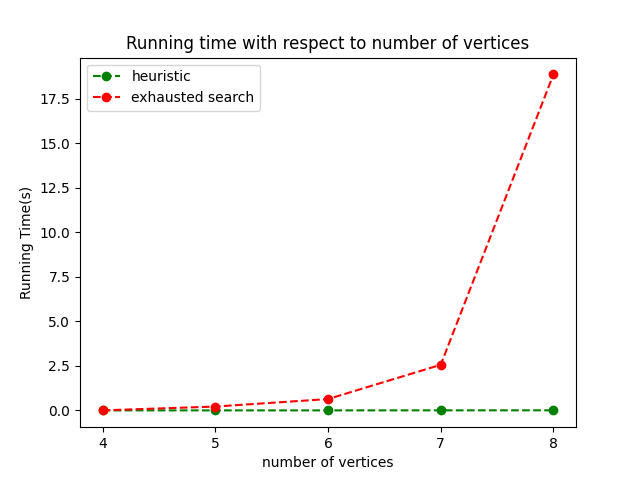
\includegraphics[width=4.2in,height=2in]{images/30_k_3.png}
    In the above chart when the graph is growing running time of the exhausted search algorithm is increasing. This is an expected result because \textbf{in bigger graphs we have more cycles} and to get k combination of that cycles \textbf{we need more time.}
\end{figure}
	
\end{projecttimeline3}

\begin{projecttimeline4}

\begin{figure}
		    
    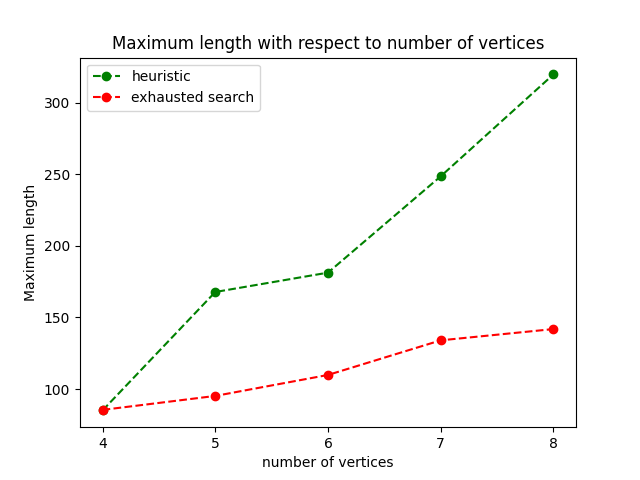
\includegraphics[width=4.2in,height=2in]{images/31.png}
    In the above chart, the heuristic algorithm gets worse results. This is an expected result because when the \textbf{k value is small} we have to \textbf{merge} the found tours. \textbf{After merging in the heuristic algorithm, the maximum length is increasing.}
    
\end{figure}
 
\end{projecttimeline4}


\begin{projecttimeline2}

In this comparison, we will change only the number of edges which means the density of the graph will change. The k value and number of nodes will be constant. We will create \textbf{20 different graphs} and we will compare the average of the results.
\newline
\newline
Parameters will be as follows.
\vspace{0.03\textheight}
\begin{itemize}
 \item \textbf{initial vertex} = 0 
 \vspace{0.02\textheight}
 \item \textbf{k} = 4
 \vspace{0.02\textheight}
 \item \textbf{number of nodes} = 6
 \vspace{0.02\textheight}
 \item \textbf{number of edges} = 7, 8, 9, 10, 11
\end{itemize}
 
\end{projecttimeline2}

\begin{projecttimeline3}

\begin{figure}
    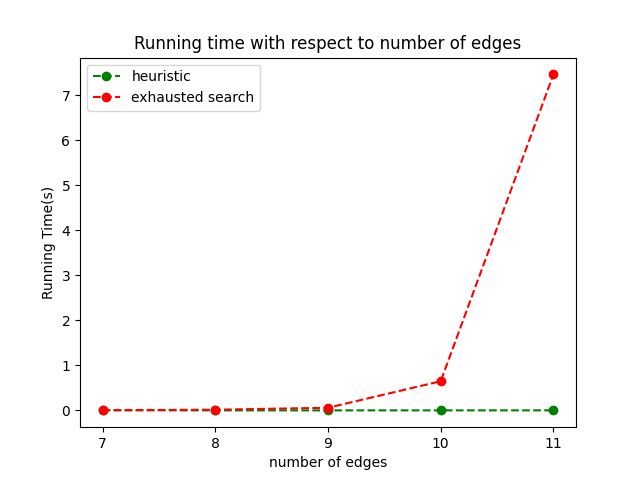
\includegraphics[width=4.2in,height=2in]{images/38.png}
    In the above chart\textbf{ when the graph density is growing} running time of the exhausted search algorithm \textbf{is increasing.} This is again an expected result because in the dense graphs \textbf{we have more cycles} and to get the k combination of that cycles \textbf{we need more time.}
\end{figure}
	
\end{projecttimeline3}

\begin{projecttimeline4}

\begin{figure}
		    
    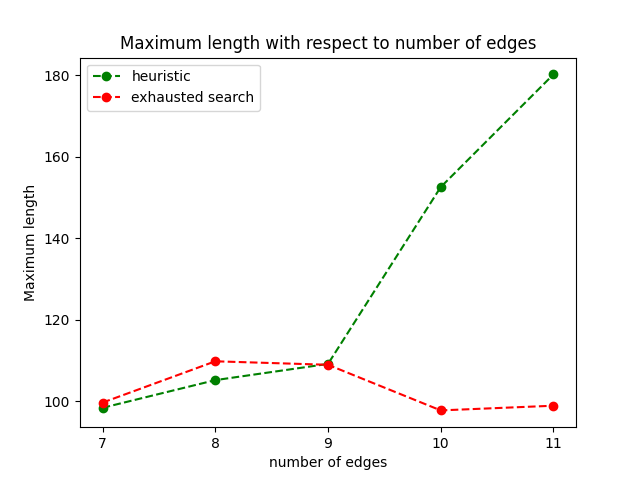
\includegraphics[width=4.2in,height=2in]{images/39.png}
    In the above chart, when the graph density is growing the heuristic algorithm gets better results, if the k value is proportional to graph size. But, \textbf{if the k value is not proportional to graph size and constant} as you can see exhausted search gets better results.
    
\end{figure}
 
\end{projecttimeline4}

\begin{projecttimeline2}

In this comparison, we will change only the k value. Number of node and number of edge will be constant. We will create \textbf{20 different graphs} and we will compare the average of the results.
\newline
\newline
Parameters will be as follows.
\vspace{0.03\textheight}
\begin{itemize}
 \item \textbf{initial vertex} = 0 
 \vspace{0.02\textheight}
 \item \textbf{k} = 5, 6, 7, 8, 9
 \vspace{0.02\textheight}
 \item \textbf{number of nodes} = 6
 \vspace{0.02\textheight}
 \item \textbf{number of edges} = 10
\end{itemize}
 
\end{projecttimeline2}

\begin{projecttimeline3}

\begin{figure}
    \includegraphics[width=4.2in,height=2in]{images/192.png}
    In the above chart when the k value is increasing running time of the exhausted search algorithm is increasing. Because the \textbf{exhausted search algorithm has to get the k combination in any case and this operation takes time.}
\end{figure}
	
\end{projecttimeline3}

\begin{projecttimeline4}

\begin{figure}
		    
    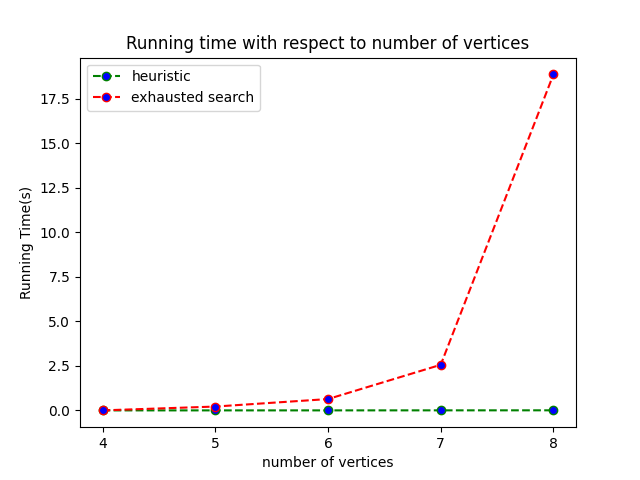
\includegraphics[width=4.2in,height=2in]{images/20.png}
    
     In the above chart when the \textbf{k value is increasing} heuristic algorithm gets \textbf{better results.} Because \textbf{when the k value is big heuristic algorithm doesn't need to merge tours} therefore it gets better results as we expect in this project.
    
\end{figure}
 
\end{projecttimeline4}

\begin{projecttimeline5}

As we have seen in the comparisons unfortunately in any case \textbf{exhausted search takes a long time.} But still, it can produce very good results. On the other hand heuristic algorithm is good for running time. But it produces bad results when the k value is small and not proportional to graph size. Because in that case, it has to make merge operation after merging the result is not good according to the exhausted search algorithm that means we can optimize the merging operating. But \textbf{when the k value is big and proportional to graph size heuristic algorithm produces better results} than the exhausted search algorithm in a very short time as we expect in this project.
 
\end{projecttimeline5}

\begin{projecttimeline6}

For this project in order to show the results and how algorithms work, we need to create a Graphical User Interface. \\
\vspace{0.02\textheight}
Features of my graphical user interface are as follows.
\vspace{0.03\textheight}
\begin{itemize}
 \item User can enter the parameter values.
 \item User can generate and see graph.
 \item User can see parallel edges as text.
 \item User can run the algorithms.
 \item User can see the algorithm results.
 \item User can see the elapsed time for each algorithm.
 \item User can see the elapsed time difference between algorithms.
 
\end{itemize}
 
\end{projecttimeline6}

\begin{projecttimeline6}

\noindent\makebox[\textwidth]{\includegraphics[width=4.9in,height=3in]{images/guit.png}}

 
\end{projecttimeline6}

\begin{projectsuccess}
\begin{enumerate}
\item Heuristic algorithm complexity will be better than $\mathcal{O}(|E|^4)$ 
\end{enumerate}
\vspace{0.03\textheight}
I have accomplished this criterion \textcolor{lightgreen}{\textbf{successfully}}. In heuristic algorithm I have $\mathcal{O}(|E|^3)$ complexity as we have seen complexity analysis. 
\end{projectsuccess}

\begin{projectsuccess}
\begin{enumerate}
\setcounter{enumi}{1}
\item Creating 50 different random graphs for each test case in performance testing and creating 20 different random graphs for each comparison case and taking the average of them.
\end{enumerate}
\begin{figure}[H]
I have accomplished this criterion \textcolor{lightgreen}{\textbf{successfully}}.
    \centering
    \subfloat[\centering Graph Generation for Heuristic Algorithm ]{{\includegraphics[width=5.5cm]{charts/12.PNG} }}%
    \subfloat[\centering Graph Generation for Exhausted Search Algorithm ]{{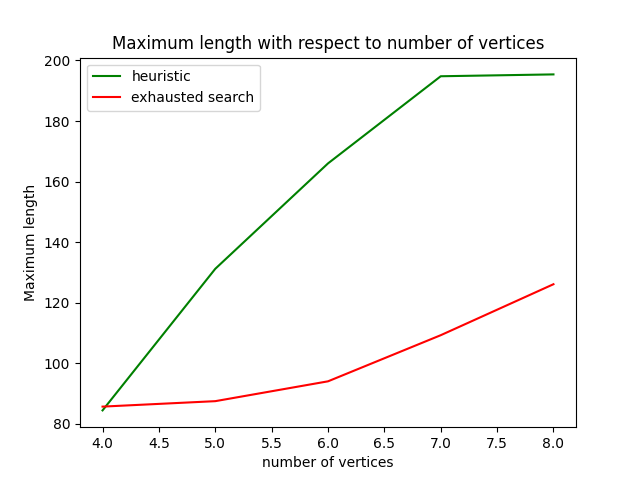
\includegraphics[width=5.5cm]{charts/11.PNG} }}%
    \caption{50 Random Graph Generation for Algorithms}
    \label{fig:ent5}
\end{figure}
\end{projectsuccess}

\begin{projectsuccess}
\begin{figure}[!htbp]
    \centering
    \includegraphics[width=3.6in,height=2.6in]{charts/13.PNG}
    \caption{\label{fig:logo}20 Random Graph Generation for Comparison}
\end{figure}
\end{projectsuccess}

\begin{projectsuccess}
\begin{enumerate}
\setcounter{enumi}{2}
\item Getting results with the heuristic algorithm in less than 1 second when number of nodes $<25$ and \textit{k} is not constant.
\end{enumerate}
\vspace{0.01\textheight}
I have accomplished this criterion \textcolor{lightgreen}{\textbf{successfully}}. As you can see in results, we have less than 1 second as running time.
\begin{itemize}
 \item \textbf{initial vertex} = 0 
 \item \textbf{number of nodes} = 8, 10, 12, 14, 16
 \item \textbf{number of edges} = $((n*(n-1)) / 2) - 5$
 \item \textbf{k} = $n*5$
\end{itemize}
\begin{figure}[!htbp]
    \centering
    \includegraphics[width=4.2in,height=0.5in]{charts/28.png}
    \caption{\label{fig:arch}Exact running time results with respect to above parameters}
\end{figure}
\
\end{projectsuccess}

\begin{projectsuccess2}
\begin{enumerate}
\setcounter{enumi}{3}
\item When \textit{k} is big and proportional to the number of edges, the results of the heuristic algorithm is at least \%4 better than the exhaustive search algorithm.
\end{enumerate}
\begin{figure}[H]
    I have accomplished this criterion \textcolor{lightgreen}{\textbf{successfully}} as we have seen in comparison.
   \subfloat[\centering When k is 7 ]{{\includegraphics[width=3cm]{charts/22.PNG} }}%
    \subfloat[\centering When k is 8 ]{{\includegraphics[width=3cm]{charts/23.PNG} }}%
    \subfloat[\centering When k is 9 ]{{\includegraphics[width=3cm]{charts/24.PNG} }}%
    \caption{Difference Calculation of Exact Results}
    \label{fig:ent5}
\end{figure}
\end{projectsuccess2}

\begin{chart4}
In this project, we have tried to solve the Minimum k-Chinese Postman Problem and we have created 2 different algorithms. 
\vspace{0.03\textheight}
\newline
While making this project, I have experienced,
\vspace{0.03\textheight}
\begin{itemize}
 \item How to make a literature search
 \vspace{0.02\textheight}
  \item How to develop and optimize algorithms
  \vspace{0.02\textheight}
 \item How to make complexity analysis and performance evaluation
 \vspace{0.02\textheight}
 \item How to compare two different algorithms and how to interpret the results
\end{itemize}

\end{chart4}

\begin{chart6}
In literature, there are a reasonable number of algorithms for this problem but finding implemented one is nearly impossible because these types of algorithms are NP-hard. Therefore implementing such algorithms is very important.
\newline
\newline
By making this project, we can help the people who are interested in these types of problems. After publishing this project people can see how to solve these types of problems, how to make a complexity analysis, and how to make a comparison between different algorithms. Also, they can use these solutions and improve them.

\end{chart6}

\begin{projecttimeline}

\begin{table}
\begin{minipage}[t]{\linewidth}
\color{gray}
\rule{\linewidth}{0.2pt}
\ytl{$1^{st} \textrm{ Meeting}$}{
\textcolor{lightgreen}{Making literature research.}\\
\textcolor{lightgreen}{Understanding the problem}}
\ytl{$2^{nd} \textrm{ Meeting}$}{
        \textcolor{lightgreen}{Continue literature research.} \\
        \textcolor{lightgreen}{Determine the steps of the heuristic algorithm.} \\
        \textcolor{lightgreen}{Start to implement heuristic algorithm}}
\ytl{$3^{rd} \textrm{ Meeting}$}{ 
    \textcolor{lightgreen}{Finish heuristic algorithm implementation.} \\
        \textcolor{lightgreen}{Make complexity analysis of heuristic algorithm.} \\
        \textcolor{lightgreen}{Test with different parameters.} \\
        \textcolor{lightgreen}{Start to implement exhaustive search algorithm}}
\ytl{$4^{th} \textrm{ Meeting}$}{
\textcolor{lightgreen}{Finish exhaustive search algorithm impl.} \\
\textcolor{lightgreen}{Make complexity analysis of e.s. algorithm.} \\
\textcolor{lightgreen}{Making comparison and numerical evaluation.} \\
\textcolor{lightgreen}{Create a graphical user interface}}
\bigskip
\rule{\linewidth}{0.2pt}%
\end{minipage}%
\end{table}
 
\end{projecttimeline}

\begin{projectreferences}

 \setlength{\emergencystretch}{1em}
\printbibliography
\addtocontents{toc}{\protect\vspace{18pt}}
\addcontentsline{toc}{chapter}{Bibliography}
 \nocite{book7,zero,Two}
\end{projectreferences}

\begin{finish}

\end{finish}

\end{document}
